\documentclass[12pt,german]{article}
\usepackage{listings}
%\usepackage[utf8]{inputenc}
\usepackage{inputenc}
\usepackage{graphicx}
\usepackage{float}
\usepackage{array}
\usepackage{pdfpages}

\lstset{
extendedchars=\true,
language=JAVA,
numbers=left, 
numberstyle=\footnotesize, 
%inputencoding=utf8,
%basicstyle=\ttfamily,
%basicstyle=\ttfamily\fontsize{8}{8},
%commentstyle=\ttfamily\fontsize{8}{8},
basicstyle=\tiny;
columns=fullflexible,
%xleftmargin=5pt,
frame=single,
breaklines=true,
postbreak=\mbox{{$\hookrightarrow$}\space},
}
\renewcommand{\thesubsubsection}{\alph{subsubsection} )}
%\renewcommand{\thesubsubsection}{\thesubsection.\alph{subsubsection} )}

\setcounter{section}{1}

\begin{document}

\title{Übungsaufgaben II, SBV1 }
\author{Lukas Fiel, Lisa Panholzer}
\maketitle


\newpage
\section{Übungsaufgaben II}
\subsection{Resampling und Interpolation}
\subsubsection{Implementierung Resampling}
Die Implementierung des Resampling Filters wurde in diesem Abschnitt anhand der Nearest Neighbour Interpolation umgesetzt. Bevor der Filter ausgeführt wird, wird zuerst der Skalierungsfaktor bei dem Benutzer abgefragt. Gibt der Benutzer einen Wert ein, der über 1.0 liegt, wird das Bild vergrößert. Gibt er einen Wert ein, der unter 1.0 liegt wird das Eingangsbild verkleinert.

In dieser Implementierung wird die Umrechnung der Koordinaten anhand der Variante B umgesetzt. Dies bedeutet, dass der Skalierungsfaktor bereits vor der Neuberechnung der Koordinaten angepasst wird, in dem von diesem 1 subtrahiert wird. Das heißt, die neue Koordinate vom skalierten Bild B wird aus der Multiplikation der Koordinate aus dem Originalbild A um den adaptierten Skalierungsfaktor s' berechnet. Dies hat zur Folge, dass sich die Indizes in der Mitte zentrieren. Der Anfang bzw. das Ende des Bild Arrays bleibt hierbei aber weiterhin unterrepräsentiert.\\

\lstinputlisting[frame=single,language=JAVA,breaklines=true]{../../Resample_.java}

\subsubsection{Implementierung Bi-Lineare Interpolation}
Die Implementierung des Resamplings Filters wurde in diesem Abschnitt anhand der Bilinearen Interpolation umgesetzt. Bevor der Filter ausgeführt wird, wird zuerst der Skalierungsfaktor bei dem Benutzer abgefragt. Gibt der Benutzer einen positiven Wert ein, der über 1.0 liegt, wird das Bild vergrößert. Gibt er einen darunterliegenden Wert ein wird das Eingangsbild verkleinert.

Danach wird die neue Höhe und Breite des Eingangsbildes anhand des Skalierungsfaktor berechnet. Zusätzlich wird der Skalierungsfaktor für die x und y Koordinaten separat berechnet und gespeichert. Anschließend wird anhand einer for-Schleife über alle Pixel des neu angelegten Arrays des skalierten Bildes iteriert. 

Neben der neuen Koordinate wird der Pixelwert anhand der Methode GetBilinearInterpolatedValue() berechnet. In dieser werden unterschiedliche Fragemente für die Berechnung des gewichteten Mittelwert aufbereitet. Damit der neue skalare Wert berechnet werden kann, müssen zuerst 4 benachbarten Pixel aus dem Originalbild ermittelt werden. Die Nachbarpixel sind folgende: p1(x+1,y), p2(x,y+t1), p3(x+1, y+1) und p4(x,y). 


Um den gewichtet Mittelwert für diesen Pixel zu erhalten werden anhand der Kalkulationsfragmente, den benachbarten skalaren Werten (p1-p4) der gewichtete Mittelwert berechnet werden. Anschließend wird dieser Wert an die Methode retourniert und im skalierten Bild an der aktuellen Koordinate eingefügt.\\

\textit{Test der Implementierung}

Um die Implementierung des Resampling Filters anhand der bi-linearen Interpolation zu prüfen, wurden zwei Testbilder inklusive Differenzbilder generiert.

Folgendes Bild wurde um den Faktor 3.0 vergrößert:

\begin{figure}[H]
	\centering
	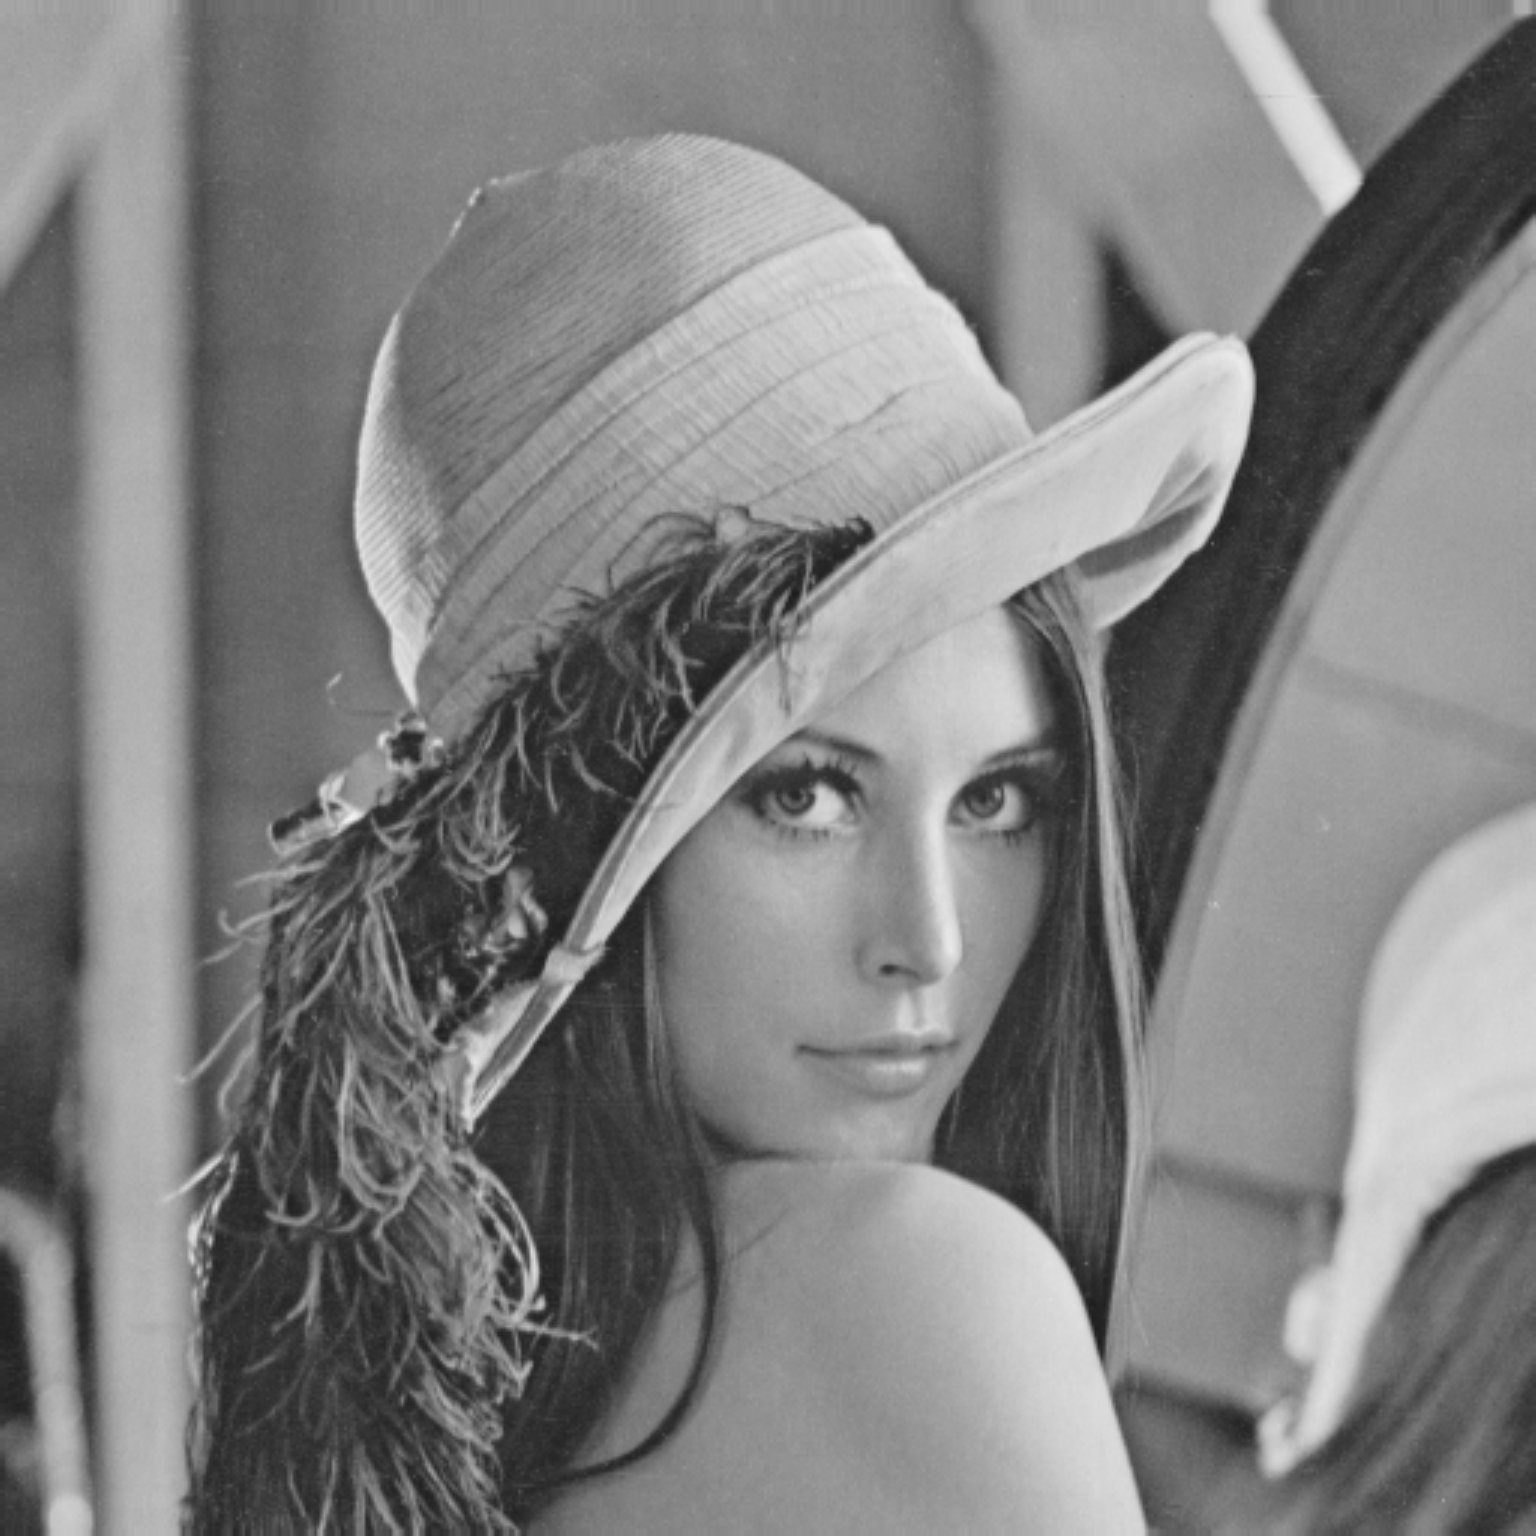
\includegraphics[width=12cm]{images/scaled-img-bilinear-interpolation-3.jpg}
	\caption{Skalierung anhand Faktor 3.0}
	\label{fig:resultResamplingBilinearInterpolation-3.0}
\end{figure}
TODO: Testbild einfügen

Testbild zur bilinearen Interpolation (Skalierungsfaktor 2.0):

\begin{figure}[H]
	\centering
	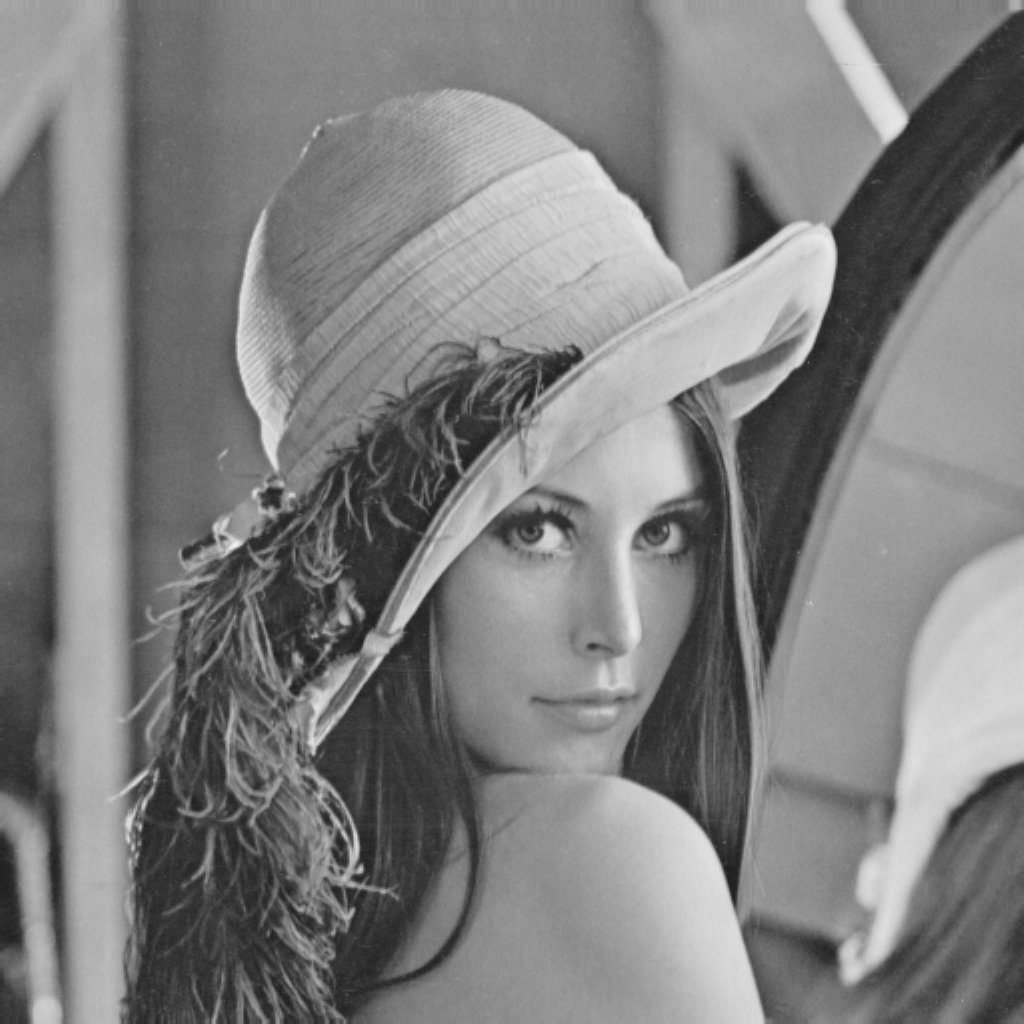
\includegraphics[width=7cm]{images/bilineare-interpolation-final/bip-scaled-2.jpg}
	\caption{Resampling anhand bilinearer Interpolation und Skalierung um Faktor 2.0}
	\label{fig:resultResamplingBilinearInterpolation-2.0}
\end{figure}

\begin{figure}[H]
	\centering
	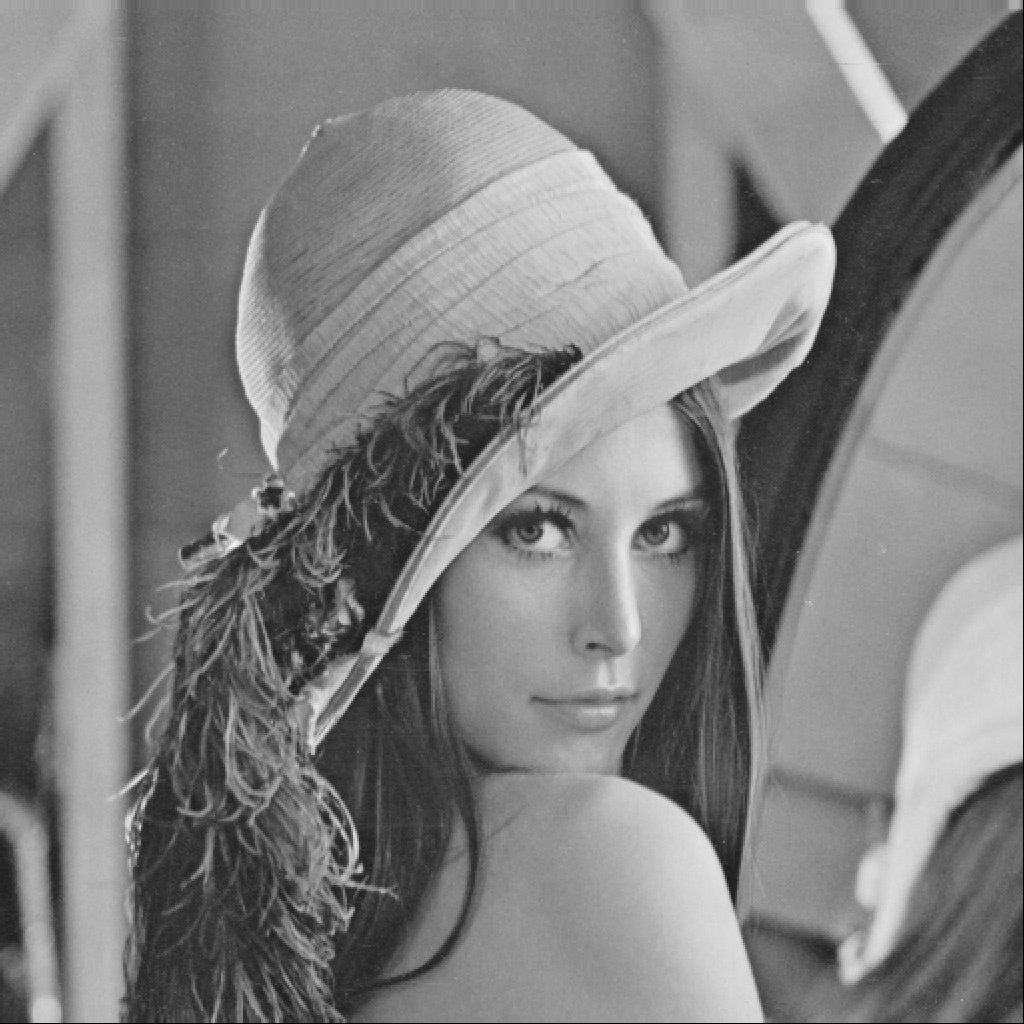
\includegraphics[width=7cm]{images/bilineare-interpolation-final/nn-scaled-2.jpeg}
	\caption{Resampling anhand Nearest Neighbor Interpolation und Skalierung um Faktor 2.0}
	\label{fig:resultResamplingNNInterpolation-2.0}
\end{figure}

\begin{figure}[H]
	\centering
	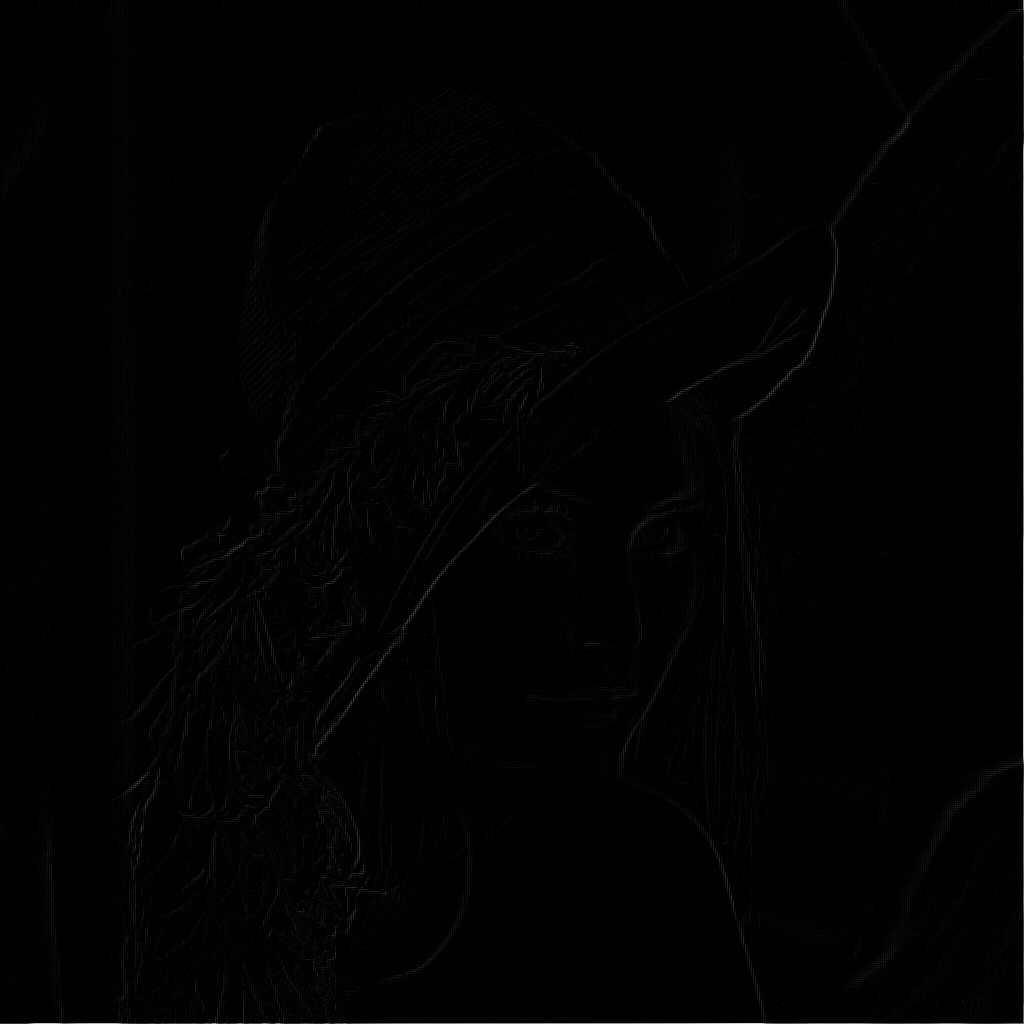
\includegraphics[width=10cm]{images/bilineare-interpolation-final/differenz-bilinear-2.jpg}
	\caption{Differenzbild generiert aus Nearest Neighbor und bilinearer Interpolation}
	\label{fig:resultResamplingDifference}
\end{figure}

Das in Figure 3 dargestellte Bild, stellt die Differenz zwischen dem Testbild das anhand der Nearest Neighbor und der bilinearen Interpolation erstellt wurde. Bei näherer Betrachtung sieht man, dass sich an den Kanten im Bild, weiße Ausprägungen wiederfinden. Dies verdeutlicht, dass die NN Interpolation aufgrund keiner Neuberechnung der Werte, diese nicht so gut wiedergibt. Diese Unterschiede in den skalaren Werten ergeben sich daraus, dass die bilineare Interpolation aufgrund der Verwendung des gewichteten Mittelwerts von 4 Pixeln einen ähnlicheren skalaren Wert ergibt, als bei der NN Interpolation.

\lstinputlisting[frame=single,language=JAVA,breaklines=true]{../../ResampleBilineareInterpolation_.java}


\subsubsection{Implementierung Checker-Board}

Die Nearest Neighbor Interpolation bezieht sich in ihrer Berechnung auf keinen neuen skalaren Wert. Es werden jeglich die benachbarten Pixel geprüft, und der Wert der am Nähesten ist, für den neuen Pixel herangezogen. Die Neuzuweisung schlägt sich auf die Bildqualität wieder, dieser wird bei einer Skalierung pixeliger bzw. kantiger.

Theoretische Überlegung: Da bei dieser Strategie kein komplexer Algorythmus verwendet wird und nur eine Neuzuweisung statt - berechnung stattfindet, ist dieser schneller als die andere Strategie.

Die bilineare Interpolation hingegen bedient sich auch der benachbarten Pixel, berechnet jedoch auf Basis dieser den gewichteten Mittelwert. Dieser Wert ist ähnlicher als zum Beispiel die Zuweisung der NN Interpolation und resuliert daher in einem besseren Bildqualität. 

Theoretische Überlegung: Aufgrund der Verwendung eines komplexeren Algorythmus ist die Laufzeit bei diesem auch länger.

 \subsection{Klassifizierung mittels Kompression}
\subsubsection{Klassifizierung von Texten}

\textbf{Idee}

Aus Texten in 8 verschiedenen Sprachen soll mittels Kompression eine Klassifizierung stattfinden. Zur Testzwecken wurden folgende Datensätze als \textit{ *.txt}  Datein in deutsch, englisch, französisch, spanisch, polnisch, ungarisch, bosnisch, und niederländisch vorbereitet:

\begin{itemize}
	\item Abstract einer wissenschaftlichen Arbeit. Diese hatte den Vorteil dass es eine deutsche und englische Übersetzung gab. Alle weiteren Sprachen wurden aus der englischen Version mittels \textit{google translate} generiert.
	\item Wörterbuch mit 10000 deutschen Wörtern. Dieser Datensatz wurde mittels \textit{google translate} in alle anderen Sprachen übersetzt.
	\item Die erste Seite der Datenschutzrichtlinien von Facebook. Da die Datenschutzrichtlinien in sämtlichen Sprachen abrufbar sind, konnte für alle Sprachen ein passender Datensatz gefunden werden.
	\item Die erste Seite der Datenschutzrichtlinien von Google. Auch hier waren Daten in allen Sprachen verfügbar.
	\item Ein Witz der aus dem deutschen mittels \textit{google translate} in alle andern Sprachen übersetzt wurde.
\end{itemize}

Zur Weiterverarbeitung wurden den Sprachen Nummern zugeordnet die man folgender Liste entnehmen kann.

\begin{itemize}
	\item 1 = bosnisch
	\item 2 = deutsch
	\item 3 = englisch
	\item 4 = spanisch
	\item 5 = französisch
	\item 6 = niederländisch
	\item 7 = polnisch
	\item 8 = ungarisch
\end{itemize}

Da nach einer Übersetzung die Texte in verschiedenen Sprachen ungleich viele Buchstaben beinhalten ist auch die Dateigröße unterschiedlich. Dies könnte eventuell rechnerisch berücksichtigt werden. Viel einfacher aber ist es, die letzten Buchstaben jedes langen Textes zu ignorieren und so eine einheitliche Länge des Textes zu gewährleisten. Dies wurde mittels eines shell-Skripts erreicht, welches nur die ersten $n$ Bytes eines Files speichert. So konnte für jeden Text eine Datei erzeugt werden die in allen Sprachen den selben Speicherbedarf hat. Der Verlust der letzten Byte ist bei einer Klassifizierung unwesentlich. 

\lstinputlisting[frame=single,language=MATLAB,breaklines=true]{../cutData.sh}

Nach einer solchen Normierung der Texte können diese miteinander verglichen werden. Dazu wurde ein Programm in \textit{Octave} geschrieben (siehe Listing \ref{fig: calculateMatrixOctaveCode}  , welches die Texte der einzelnen Datensätze miteinander vergleicht und in einer Matrix darstellt. Eine qualitativ hochwertige Aussage ob die Ergebisse statistische Aussagekraft haben, kann mit $5$ Datensätzen nicht getroffen werden. Es ist aber sicherlich ein Trend erkennbar.


\begin{figure}[H]
	\centering
	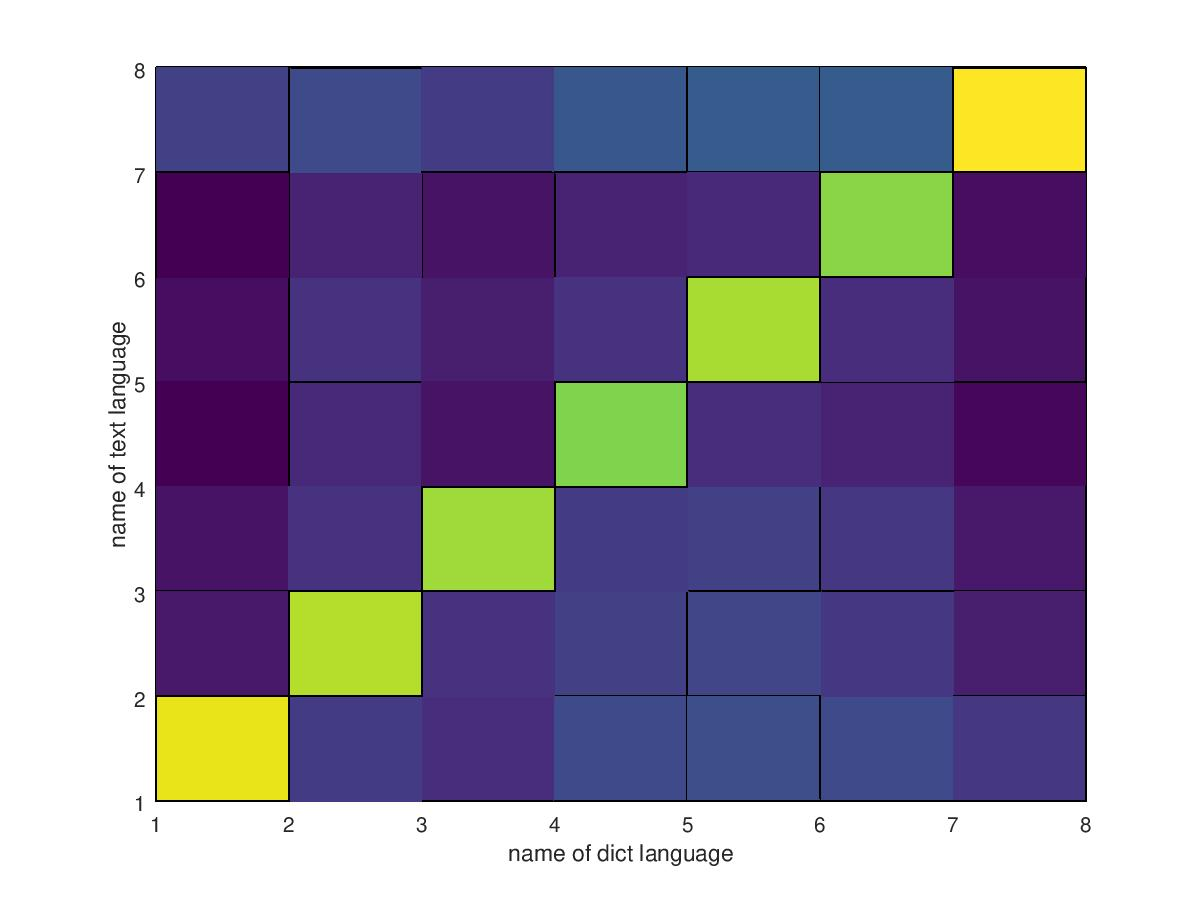
\includegraphics[width=12cm]{images/resultZipData.jpg}
	\caption{zipDataMatrix}
	\label{fig: zipDataMatrix}
\end{figure}

\newpage
\lstinputlisting[frame=single,language=MATLAB,breaklines=true,caption = Octave Script zur Darstellung der einzelnen Kompressionsraten.]{../calculateZipMatrix.m}
\label{fig: calculateMatrixOctaveCode}


\subsubsection{OPTIONAL – nur für Interessierte/Experten}


\subsection{Kompression und Code-Transformation}
\subsubsection{Lempel-Ziv Kompression einer Sequenz}
Figure \ref{fig: manualLemperZivPdf} zeigt die händische Berechnung der Lemper Ziv Kompression. Beim Übertragen ins Protokoll wurde allerdings ein Fehler entdeckt, der in Tabelle \ref{tab:Level Ziv Kompression} korrigiert wurde.



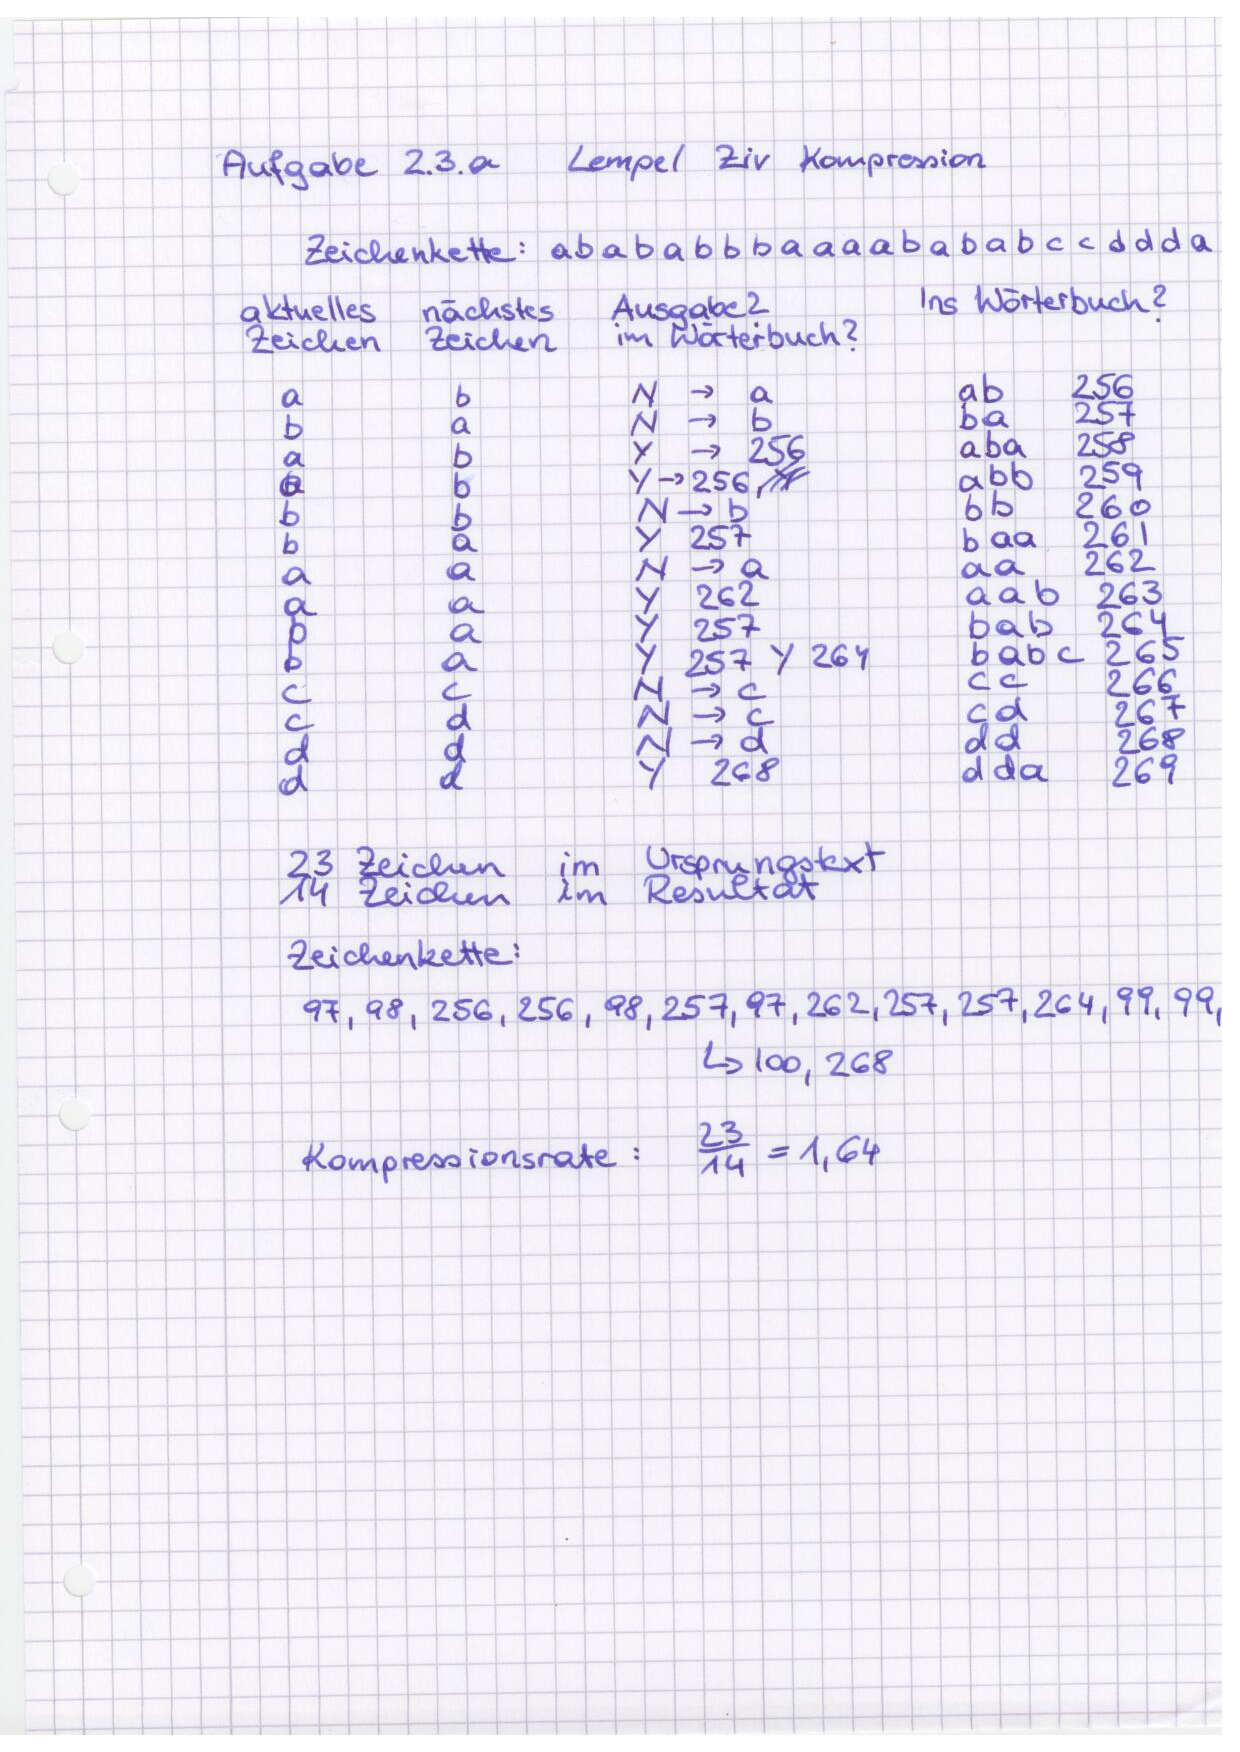
\includepdf[scale=0.4]{images/lemperZiv.pdf}
\label{fig: manualLemperZivPdf}


\begin{table}[H]
  \centering
  \begin{tabular}{c | c | c | c | c |}
    \hline
   	aktuelles  & nächstes  & Ausgabe  & ins & Speicher \\
   	 Zeichen &  Zeichen &  (im Wörterbuch?) & Wörterbuch! &  \\
	a & b & N $ \rightarrow $ a & ab & 256 \\
	b & a & N $ \rightarrow $ b & ba & 257 \\
	a & b & Y $ \rightarrow $ 256 & aba & 258 \\
	a & b & Y $ \rightarrow $ 256 & abb & 259 \\
	b & b & N $ \rightarrow $ b & bb & 260 \\
	b & a & Y $ \rightarrow $ 257 & baa & 261 \\
	a & a & N $ \rightarrow $ a & aa & 262 \\
	a & a & Y $ \rightarrow $ 256 & aab & 263 \\
	b & a & Y $ \rightarrow $ 257 & bab & 264 \\
	b & a & Y (257), Y $ \rightarrow $ 264 & babc & 265 \\
	c & c & N $ \rightarrow $ c & cc & 266 \\
	c & d & N $ \rightarrow $ c & cd & 267 \\
	d & d & N $ \rightarrow $ d & dd & 268 \\
	d & d & Y $ \rightarrow $ 268 & dda & 269 \\
	a &   & N $ \rightarrow $ a &     &   \\ 
   	
  \end{tabular}
  \caption{Level Ziv Kompression}
  \label{tab:Level Ziv Kompression}
\end{table}

In der korrigierten Version ergibt die resultierende Zeichenkette: 

\begin{table}[H]
  \centering
  \begin{tabular}{| c | c | c | c | c | c | c | c | c | c | c | c | c | c | c |}
    \hline
    97 & 98& 256 & 256 & 98 & 257 & 97 & 262 & 257 & 264 & 99 & 99 & 100 & 268 & 269 \\
    \hline
  \end{tabular}
\end{table}


\begin{equation}[H]
 Kompressionsrate C = \frac{23}{15} = 1.5334	
\end{equation}


\subsubsection{Huffmann Coding}

Die nächste Seite zeigt die händische Berechnung des Huffmann Baums zum gegebenen Beispiel. Die mittlere Codewortlänge lieght dabei bei $1.869 bit $. \\

Weiters kann man auf der darauffolgenden Seite die manuelle Berechnung von 6 Testfällen finden. Es kann gesagt werden, dass die Huffmann Kompression sehr gut geeignet wäre um Daten zu komprimieren, die sehr oft gleich sind. Dabei spielt homogenität keine Rolle, sondern rein die Häufigkeit des Auftretens der Sonderfälle. An diser Stelle sei erwähnt, dass die Information über solche Sonderfälle nicht verloren geht, sondern einfach mehr Speicher benötigt (verlustfreies Komprimieren).

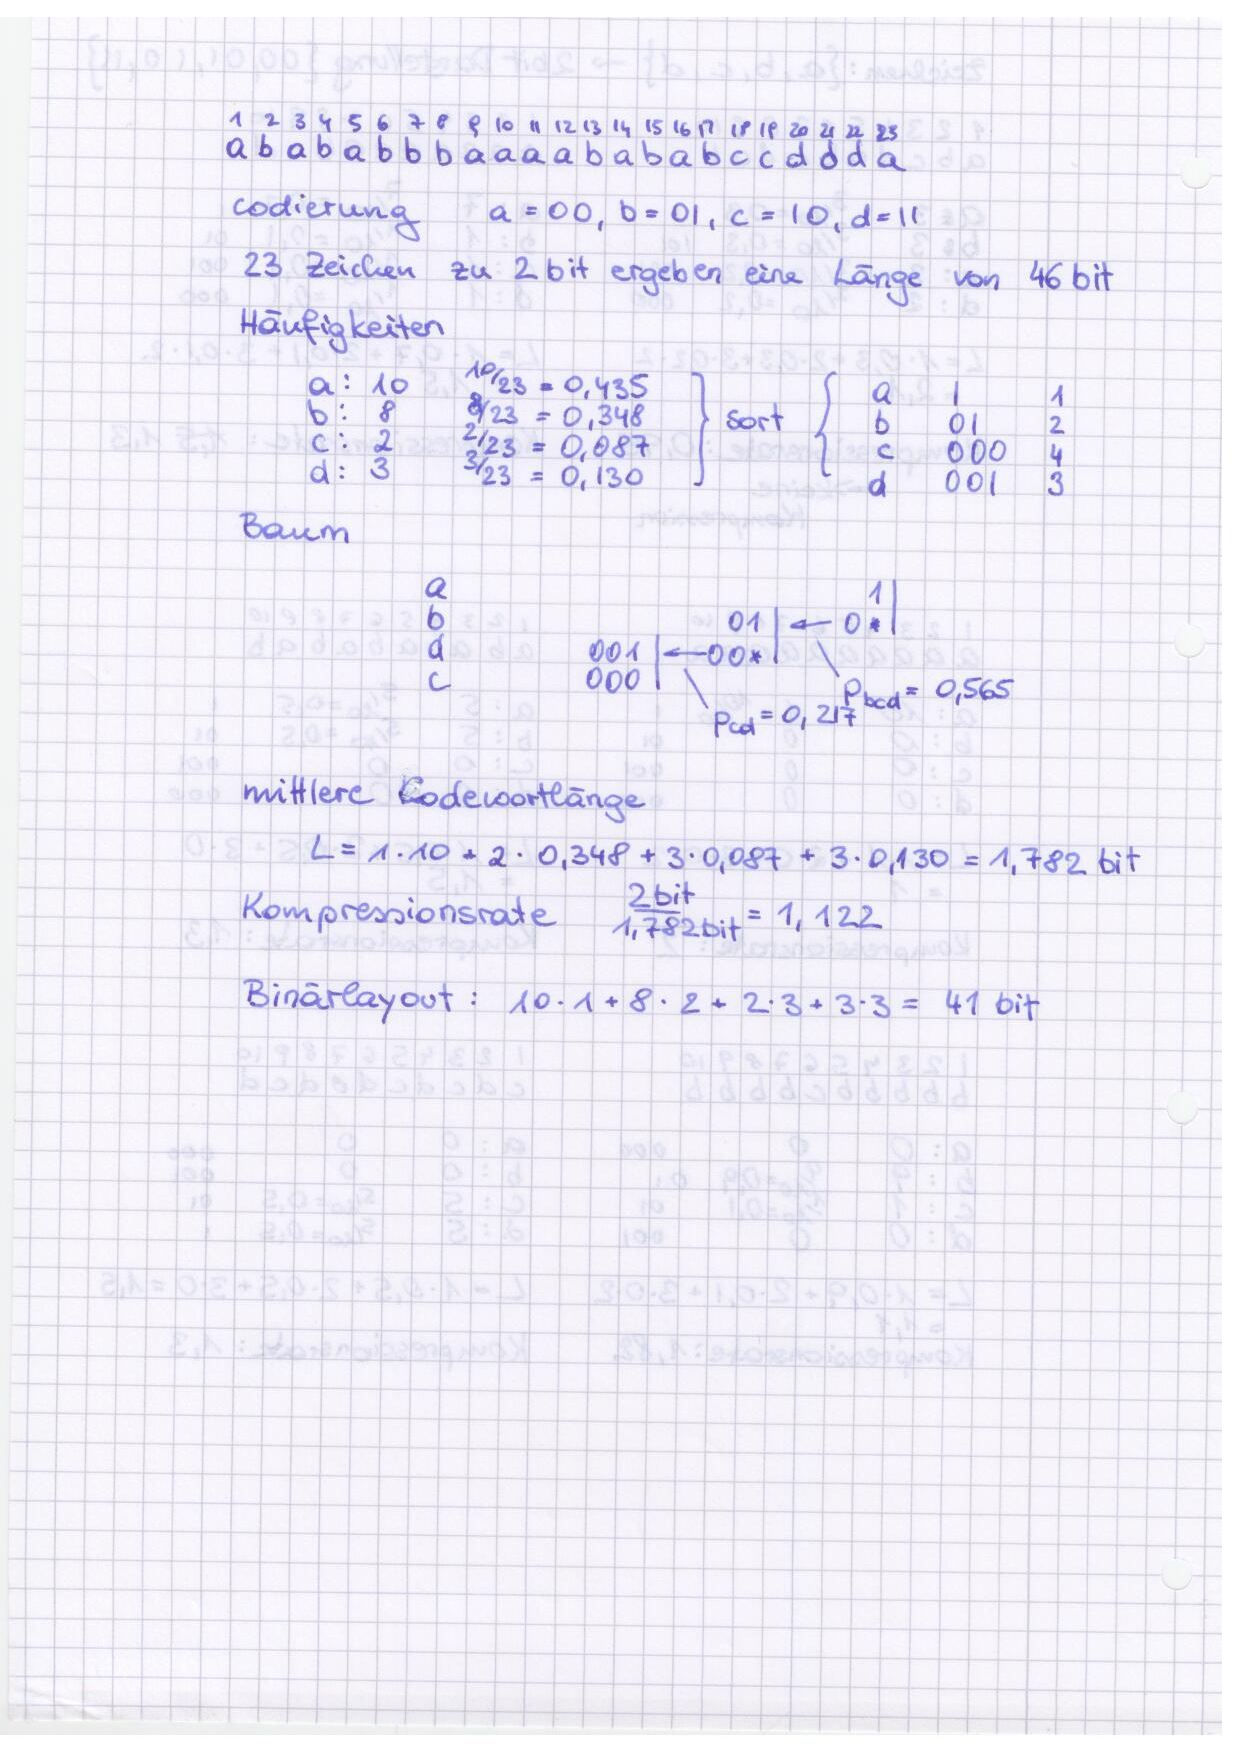
\includepdf{images/huffmannBerechnung.pdf}
\label{fig:huffmannCalculation}

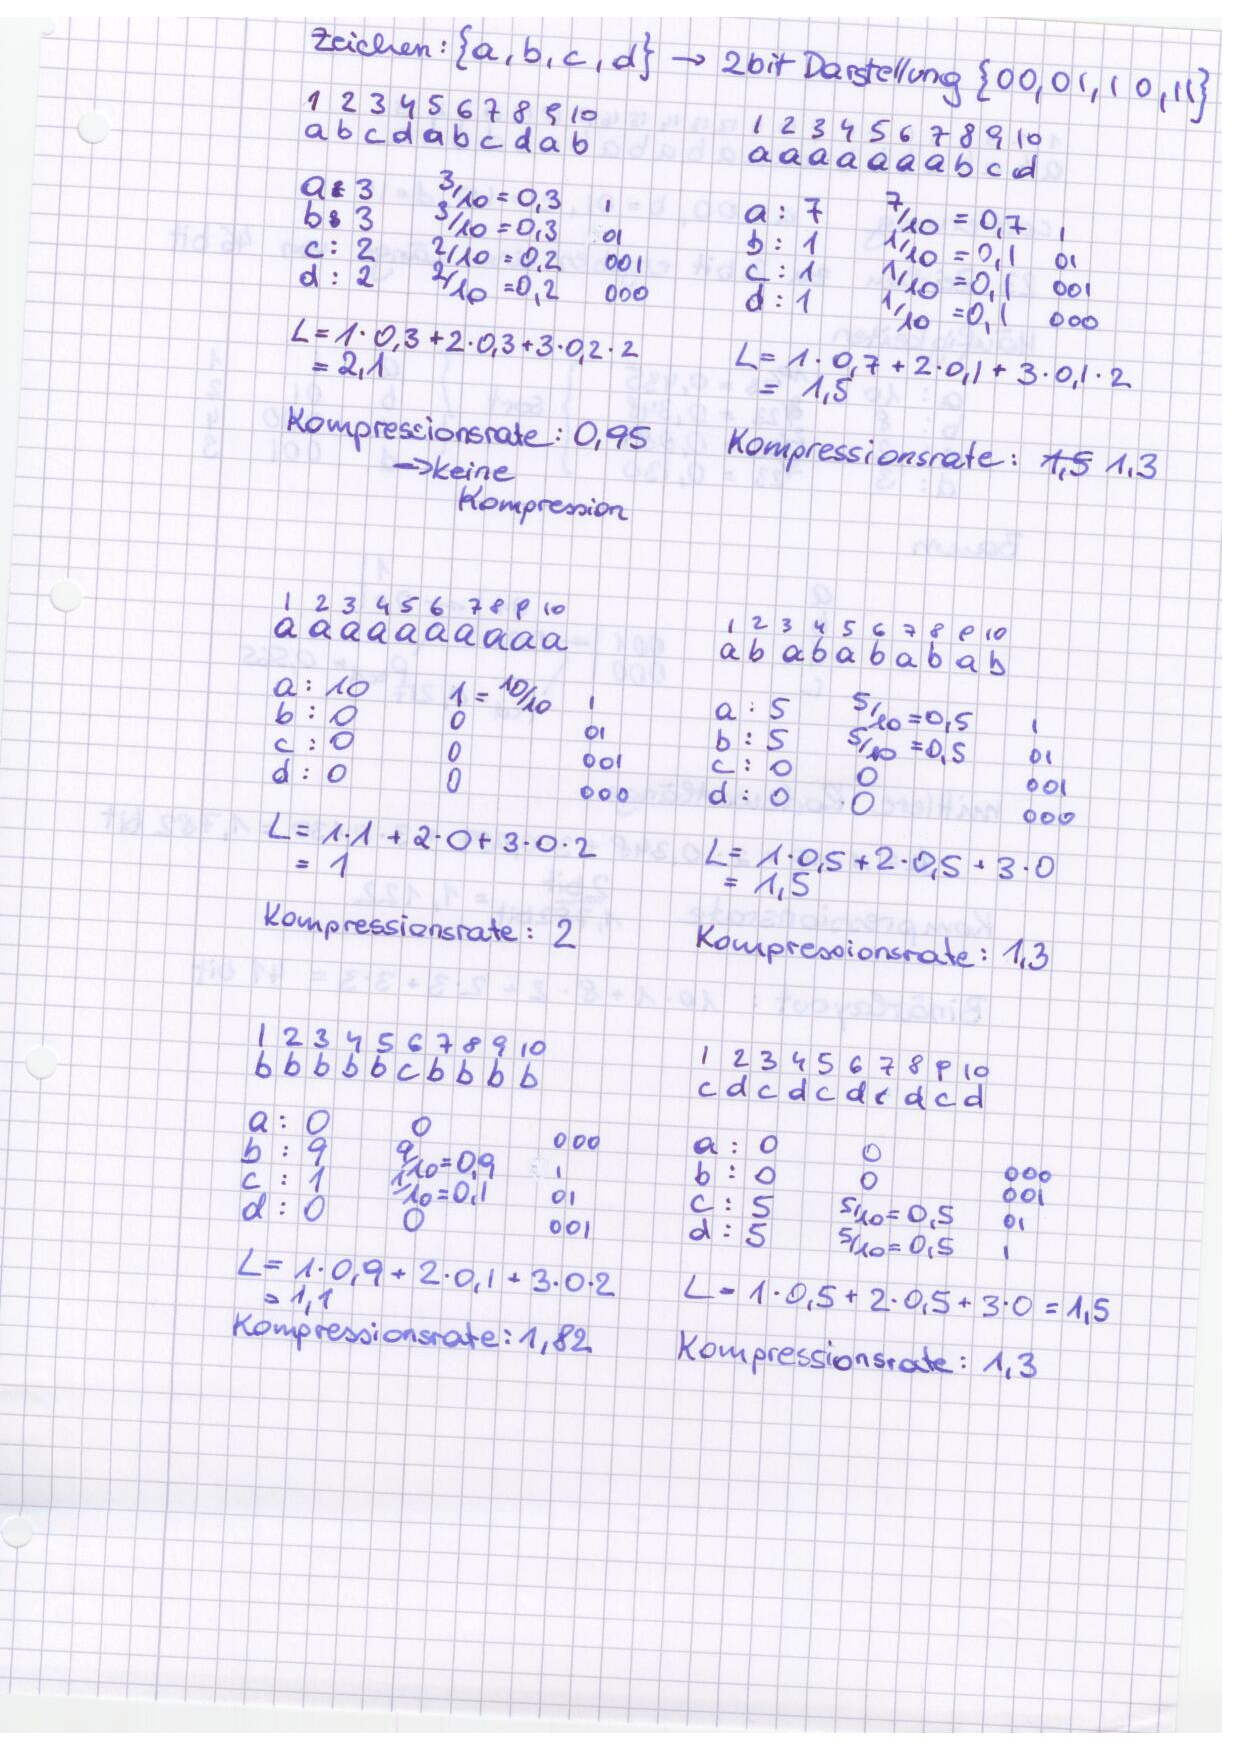
\includepdf{images/huffmannTestfaelle.pdf}
\label{fig:huffmannCalculation}


\subsubsection{Komprimierung einer Sequenz mittels Runlength Coding}
\textit{Berechnung der Kompressionsrate} 

Die nachfolgende Sequenz soll anhand von Runlength Coding händisch komprimiert und die Kompressionsrate ausgegeben werden:

010101111100000111100010101111 (30 Stellen, n=2 Symbole:0,1) \\

Die Sequenz wird von links nach rechts codiert, und anstatt der eigentlichen Zeichen die Häufigkeit dieser ausgegeben. Nach der händischen Komprimierung weist die Frequenz folgende Lauflänge auf:

11111554311114 (14 Stellen)\\


Daraus ergibt sich folgende Kompressionsrate:

30/14 = \textbf{ 2,14}\\

\textit{Erweiterung der Symbolmenge}\\
Die Komprimierung von Sequenzen anhand der RLC ist am effektivsten, je homogener der Informationsgehalt ist. Das bedeutet, das bei vielen unterschiedlichen Zeichen die Komprimierungsmethode nicht mehr sinnvoll angewandt werden kann. Bei sehr kurzen Sequenzen kann es sogar zu einer Erhöhung der Zeichenanzahl in dieser kommen.\\

Wird nun die Anzahl der Symbole erhöht, muss beachtet werden, dass zusätzlich zu der Häufigkeit des Zeichens noch ein Trennsymbol, eine ID bzw. das Zeichen selbst mitgegeben werden muss. Dies wird anhand eines selbst gewählten Beispiels demonstriert.\\

Folgende Sequenz wird anhand von RLC komprimiert:

AAZZBBBBBBBBCCCCCCCDEEEEEEEFFGHIIJJJKLMN\\ (40 Stellen, n=14 Symbole:A,Z,B,C,D,E,F,G,H,I,J,K,L,M,N)\\

Die komprimierte Sequenz lautet:

A2Z2B8C7D1E7F2H1I2J3K1L1M1N1 (28 Stellen)\\

Daraus ergibt sich folgende Kompressionsrate:

40/28=\textbf{1,42}\\

Wird eine sehr kurze Sequenz mit einer hohen Anzahl an Symbolen komprimiert, kann es aufgrund des hohen Informationsgehalts dazu kommen, dass die codierte Sequenz länger ist, als die Originale.\\


Folgende Sequenz wird anhand von RLC komprimiert:

AZBBCDEEFFFGHIIJJJKLLLMNOPQRSTU\\ (30 Stellen, n=21 Symbole:A,Z, B,C,D,E,F,G,H,I,J,K,L,M,N,O,P,Q,R,S,T)\\

Die komprimierte Sequenz lautet:

A1Z1B2C1D1E2F3G1H1I2J3K1L3M1N1O1P1Q1R1S1T1 (42 Stellen)\\

Daraus ergibt sich folgende Kompressionsrate:

30/42=\textbf{0,71}\\

\subsubsection{Entropieberechnung}
Folgende Sequenz zur Entropieberechnung ist gegeben:

111122661112233334564511211111 (30 Stellen, n=6 Symbole: 1,2,3,4,5,6)\\

\begin{figure}[H]
	\centering
	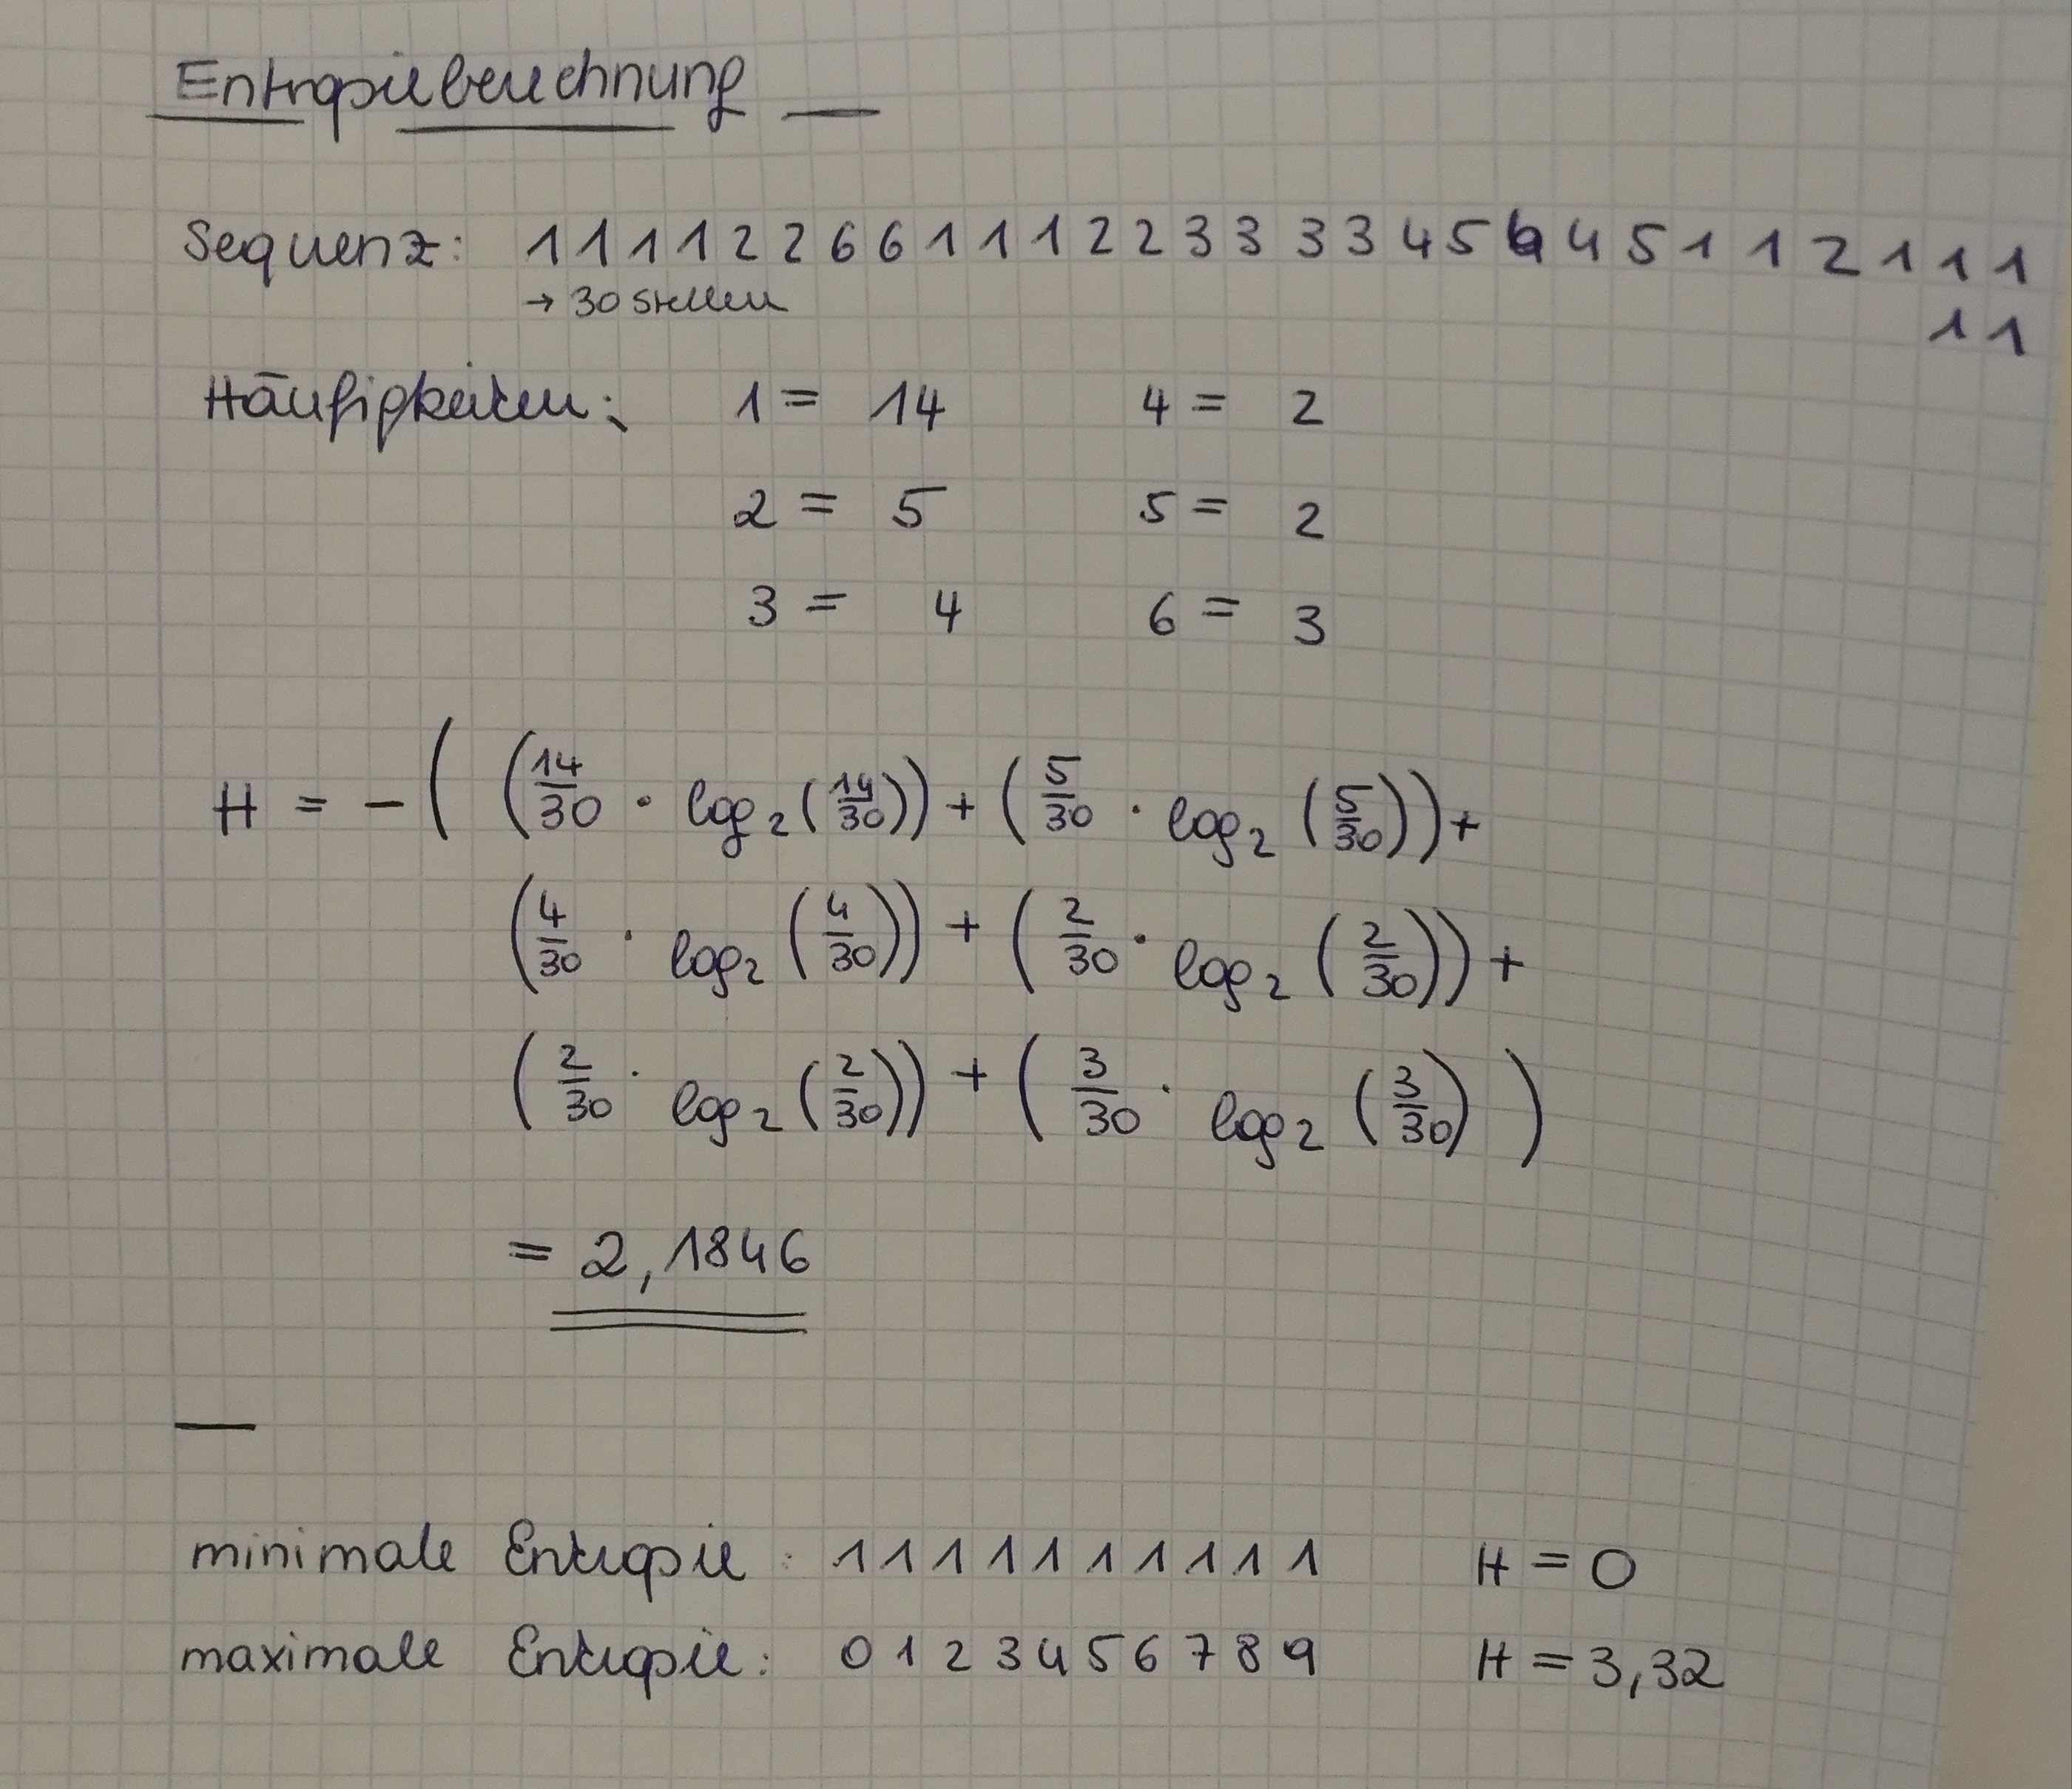
\includegraphics[width=12cm]{images/entropieBerechnung.jpg}
	\caption{manuelle Entropieberechnung}
	\label{fig:resultEntropie}
\end{figure}

Nachdem die Häufigkeiten der Symbole erfasst wurde, wurde die Formel der Shannon-Entropie angewandt. Das Ergebnis der Berechnung lautet \textbf{2,1846}. \\

\textit{Minimale und Maximale Entropie}

Bei foglender 10-stelliger Sequenz ist die Entropie minimal:

Sequenz: 1111111111 (10 Stellen, n=1 Symbol: 1)

H = 0\\

Bei folgender 10-stelliger Sequenz ist die Entropie maximal:

Sequenz: 0123456789 (10 Stellen, n=10 Symbole: 0,1,2,3,4,5,6,7,8,9)

H = 3,32\\

\textit{Auswirkung auf Kompressionsrate}\\

Eine geringe Entropie bewirkt, dass die Sequenz besser komprimierbar ist.  Je höher die Entropie, desto schlechter ist die Sequenz komprimierbar. Nicht nur die Auftrittswahrscheinlichkeit hat eine Auswirkung auf die erzielbare Kompressionsrate. Auch die Länge der Sequenz, sowie die Anzahl der Zeichen spielt eine wesentliche Rolle. Je größer diese Faktoren, desto schlechter ist eine Sequenz durch unterschiedliche Kompressionsverfahren bearbeitbar.



\end{document}
